\section{Introduction}
 
In general,  we don't need  complete information about the system as  
to check its certain property.  An additional information about the system can slow  the whole process
down or even make it infeasible. In this theory we define constraints that allow to find/check
the minimal model (and the minimal extent of the system)
needed to verify a specific property.  
Our approach focuses on data
dependencies between system components. Dependencies' analysis results in a
decomposition that gives rise to a logical system architecture, which is the most appropriate for the
case of remote monitoring, testing and/or verification.


Let  $CSet$  be a set of components  
on a certain abstraction level $L$ of logical architecture 
(i.e. level of refinement/decom\-po\-sition, data type \emph{AbstrLevelsID} in our Isabelle formalisation).
We denote the sets of input and
output streams of a component $S$ by $\instreams(S)$ (function \emph{ IN ::  CSet $\Rightarrow$ chanID set} in Isabelle) and
$\outstreams(S)$ (function \emph{ OUT ::  CSet $\Rightarrow$ chanID set} in Isabelle).
The set of local variables of components is defined in Isabelle by VAR, and the function to map component identifiers to  the corresponding variables is defined by 
\emph{ VAR ::  CSet $\Rightarrow$ varID set}. 

Please note that concrete values for these functions cannot be specified in general, because they strongly depend on a concrete system. 
In this paper we present a small case study in the theories \emph{DataDependenciesConcreteValues.thy} (specification of the system architecture on several abstraction levels) 
and \emph{DataDependenciesCaseStudy.thy} (proofs of system architectures' properties).

Function \emph{ subcomp ::  CSet $\Rightarrow$ CSet set}  maps components to a (possibly empty) set of its subcomponents. 

We specify the components' dependencies by the  function 
\[
Sources^{L}: CSet^{L} \to  (CSet^{L})^*
\]
which returns for any component identifier $A$ the corresponding (possibly
empty) list of components (names) $B_1, \dots, B_{AN}$ that are the
sources for the input data streams of $A$ (direct or indirect):
\[
\begin{array}{l}
Sources^{L}(C) = \\
DSources^{L}(C)\ \cup\  \bigcup_{S \in  DSources^{L}(C)} \{  S_1 \mid S_1 \in  Sources^{L}(S) \} 
\end{array}
\]   
%
Direct data dependencies are defined by the function 
\[
DSources^{L}: CSet^{L} \to  (CSet^{L})^*
\]
\[ 
DSources^{L}(C) = 
\{  S \mid  \exists x \in \instreams(C) \wedge x \in \outstreams(S) 
\}  
\]
 %
\newpage 
For example, 
$C_1 \in DSources^{L}(C_2)$ means that at least one of the output channels of  $C_1$ 
is directly connected to some of input channels of   $C_2$.


$\idep(C, y)$ denotes the subset of $\instreams(C)$ that output channel $y$ depends upon, 
directly (specified in Isabelle by function \emph{ OUTfromCh::  chanID $\Rightarrow$ chanID set}
  or vial local variables (specified by function \emph{ OUTfromV::  chanID $\Rightarrow$ varID set}). 
For example, let the values of the output
channel $y$ of component $C$ depend only on the
value of the local variable $st$ that represents the current state of
$C$ and is updated depending to the input messages
the component receives via the channel $x$, then $\idep(C, y) = \{ x \}$.   
In Isabelle, $\idep(C, y)$  is specified by function \emph{ OUTfrom::  chanID $\Rightarrow$ varID set}.

Based on the definition above, we can decompose system's components to have for each component's output channel 
the minimal subcomponent  computing the corresponding results (we call them \emph{elementary components}). 
An elementary component either 
\begin{itemize}
\item
should have a single output channel (in this case this component can have no local variables), 
or 
\item
all it output channels are correlated, i.e. mutually depend on the same local variable(s).
\end{itemize}
%
If after this
decomposition a single component is too complex, we can apply the
decomposition strategy presented in~\cite{spichkova2011decomp}.
 
For any component $C$, the dual function $\odep$ returns the
corresponding set $\odep(C,x)$ of output channels depending on input
$x$. This is useful for tracing, e.g., 
if there are some changes in the specification, properties, constraints, etc.\ for $x$, 
we can trace which other channels can be affected by these changes.
 
%
If the input part of the component's interface is specified correctly in the
sense that the component does not have any ``unused'' input channels, the following relation
will hold: $ \forall x \in \instreams(C). ~ \odep(C, x) \neq
\emptyset $.

We illustrate the presented ideas by a small case study:   
we show how system's components can be decomposed to optimise
the data dependencies within each single component, and after that we optimise architecture of the whole system. 
System
$S$ (cf.\ also Fig.~\ref{fig:example_comm1}) has 5 components, the set $CSet$ on the level $L_{0}$ is
defined by $\{A_1, \dots, A_9\}$. 
The sets $\idep$ of data dependencies between the components are defined in the theory \emph{DataDependenciesConcreteValues.thy}. 
We represent the dependencies graphically using dashed lines over the component box.  

\begin{figure}[ht!]
  \begin{center}
   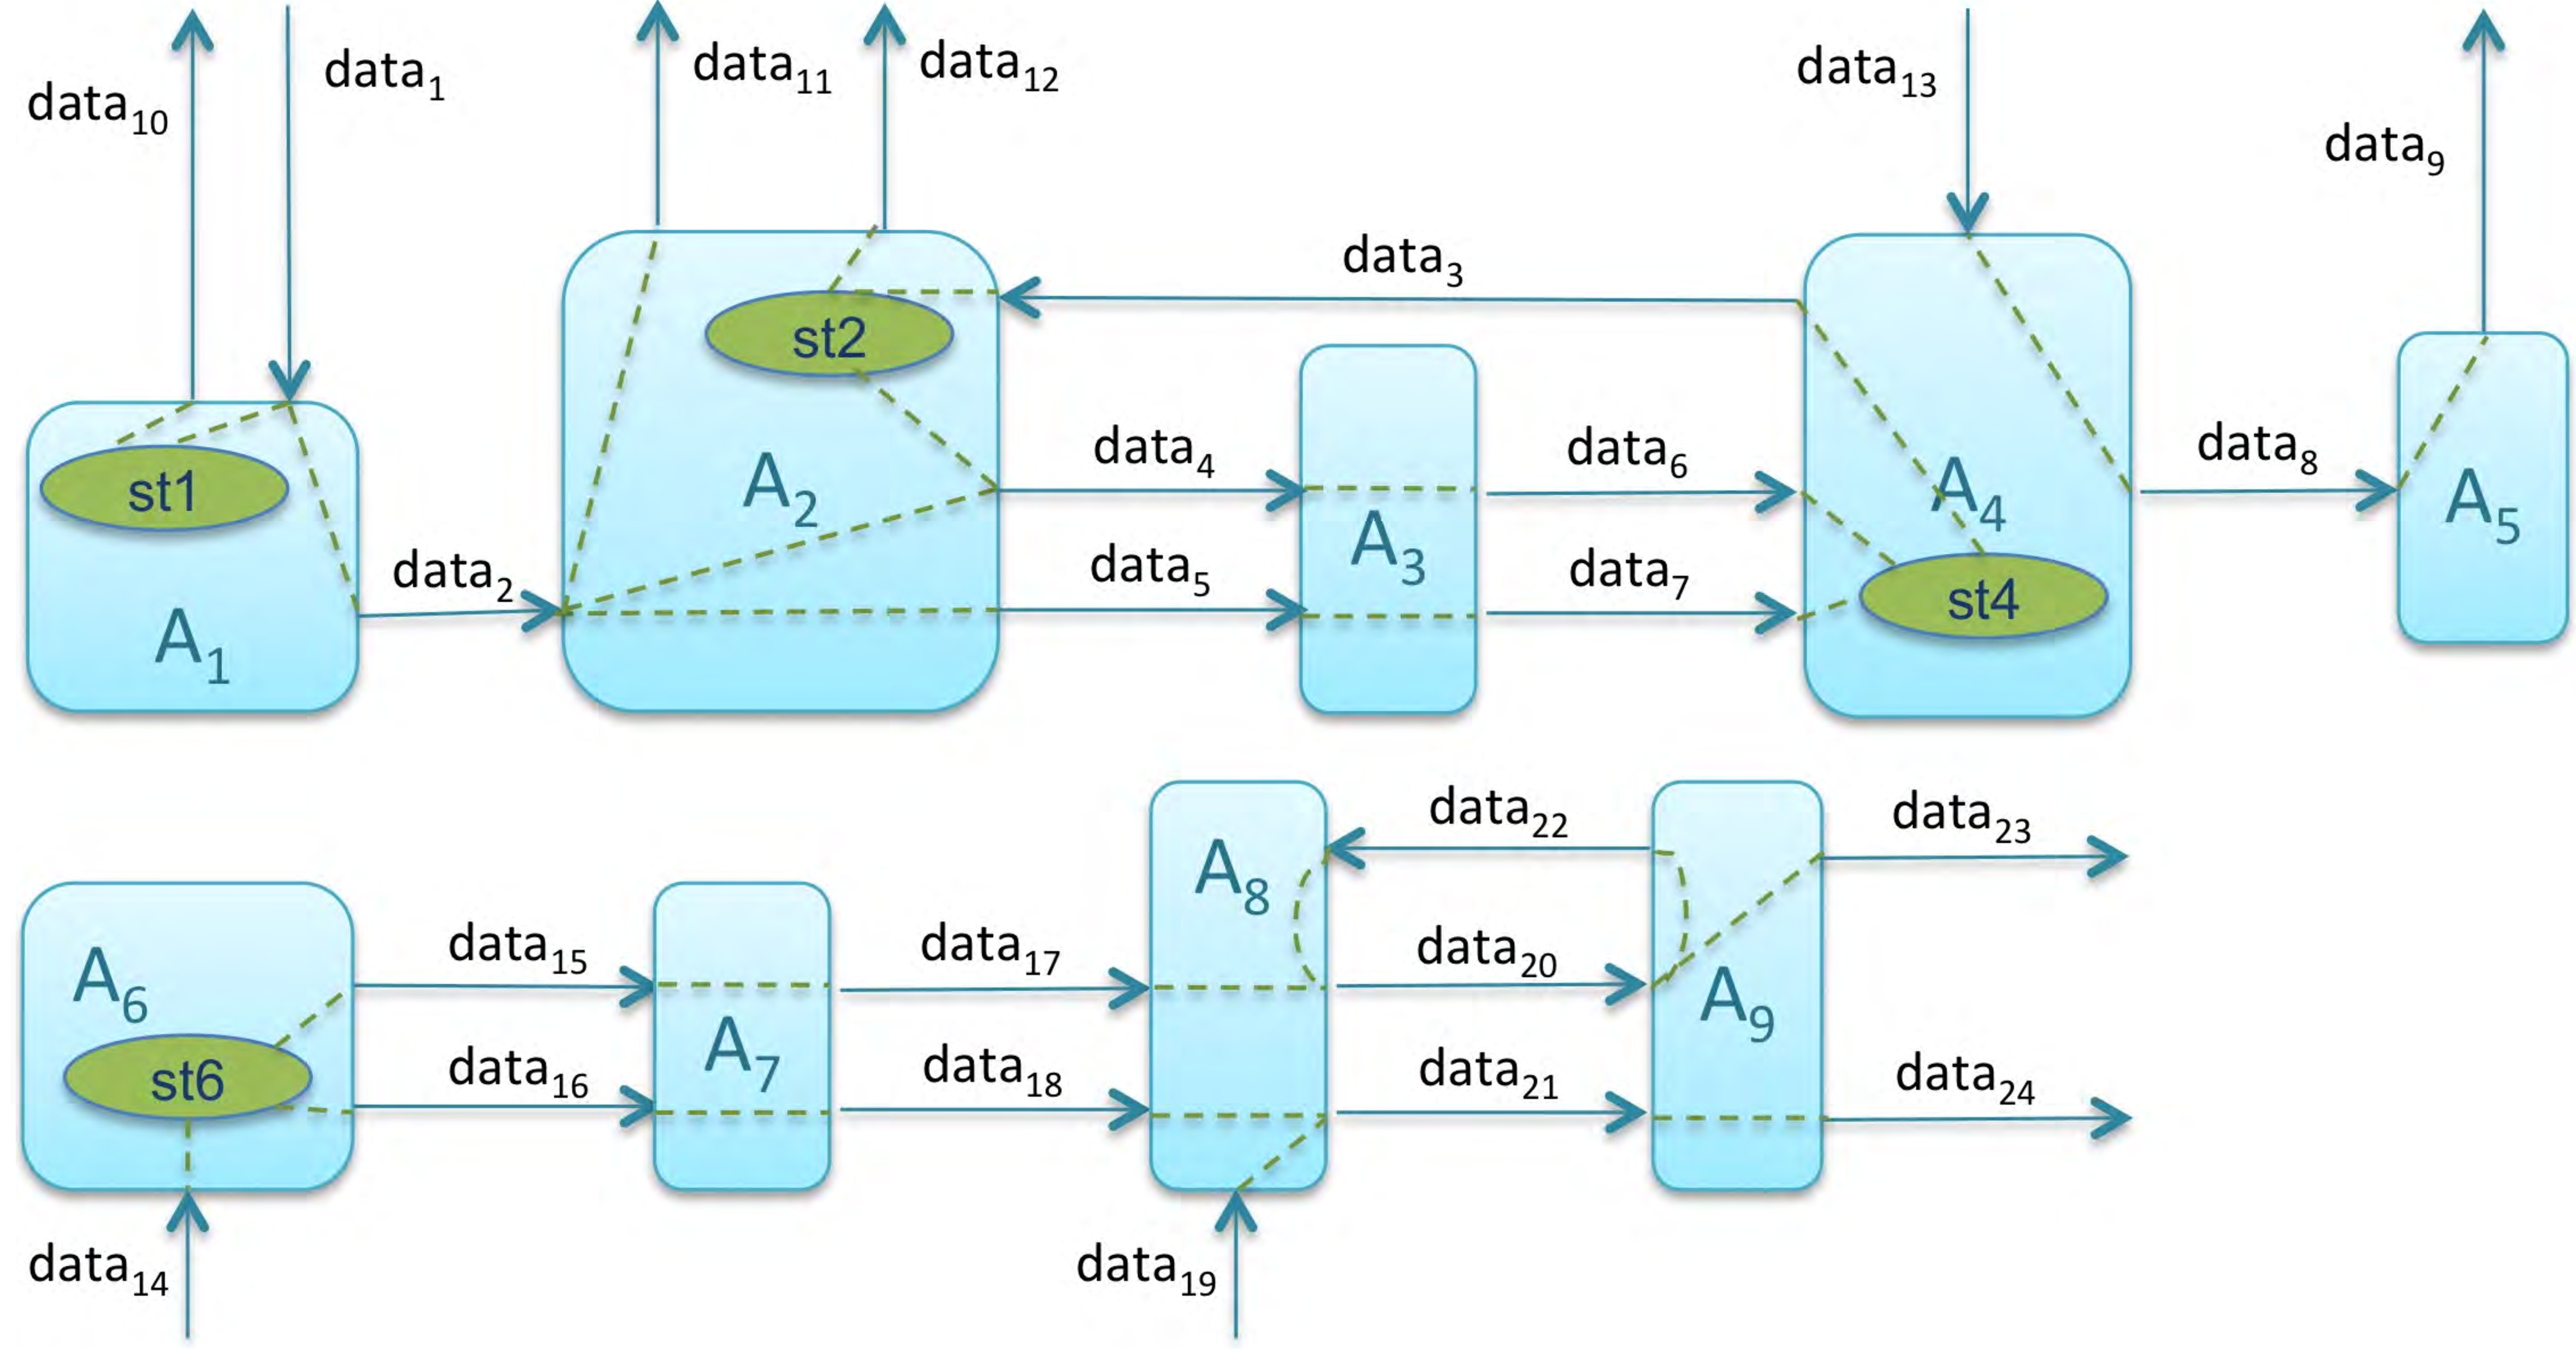
\includegraphics[scale=0.15]{fig/L0.pdf}% 
   \vspace{-3mm}
    \caption{System  $S$: Data dependencies and $\idep$ sets 
    }
    \label{fig:example_comm1}
  \end{center}
\end{figure}
 
 \newpage 
 Now we can decompose the system's components according to the given  $\idep$ specification. This results into the next abstraction level $L_{1}$ of logical architecture (cf. Fig.~\ref{fig:example_comm2}), on which all components are elementary. Thus, we obtain a  (flat) architecture of system. 
 The main feature of this architecture is that  each output channel (within the system) 
belongs the minimal subcomponent of a system computing the corresponding results. 
 We represent this (flat) architecture  as a directed graph (components become vertices and channels become edges)  
and apply one of the existing distributed algorithms for the 
decomposition into its   strongly connected components,  e.g. FB~\cite{idetifyingSSCs}, OBF~\cite{OBF}, or the colouring algorithm~\cite{Orzan04ondistributed}.
Fig.~\ref{fig:L2a} presents the result of the architecture optimisation.

After optimisation of system's architecture, we can find the minimal part of the system
needed to check a specific property (cf. theory \emph{DataDependencies}).  
A property can be represented  by relations over data flows on the system's channels, 
and first of all we should check the property itself, whether it reflect a real relation within a system. 
Let for a relation $r$, $I_{r}$ $O_{r}$ be the sets of input and output channels of the system used in this relation.
For each channel from $O_{r}$ we recursively compute all the sets of the dependent components and corresponding 
input channels. 
Their union, restricted to the input channels of the system, 
 should be equal to $I_{r}$, otherwise we should check whether the property was specified correctly. 

Thus, from $O_{r}$ we obtain the set $outSetOfComponents$ of components having these channels as outputs, and
compute the union of corresponding sources' sets.
This union together with $outSetOfComponents$ give us  the minimal part of the system 
needed to check the property $r$: we formalise it in Isabelle  by the predicate $minSetOfComponents$.  


 

\begin{figure}[ht!]
  \begin{center}
   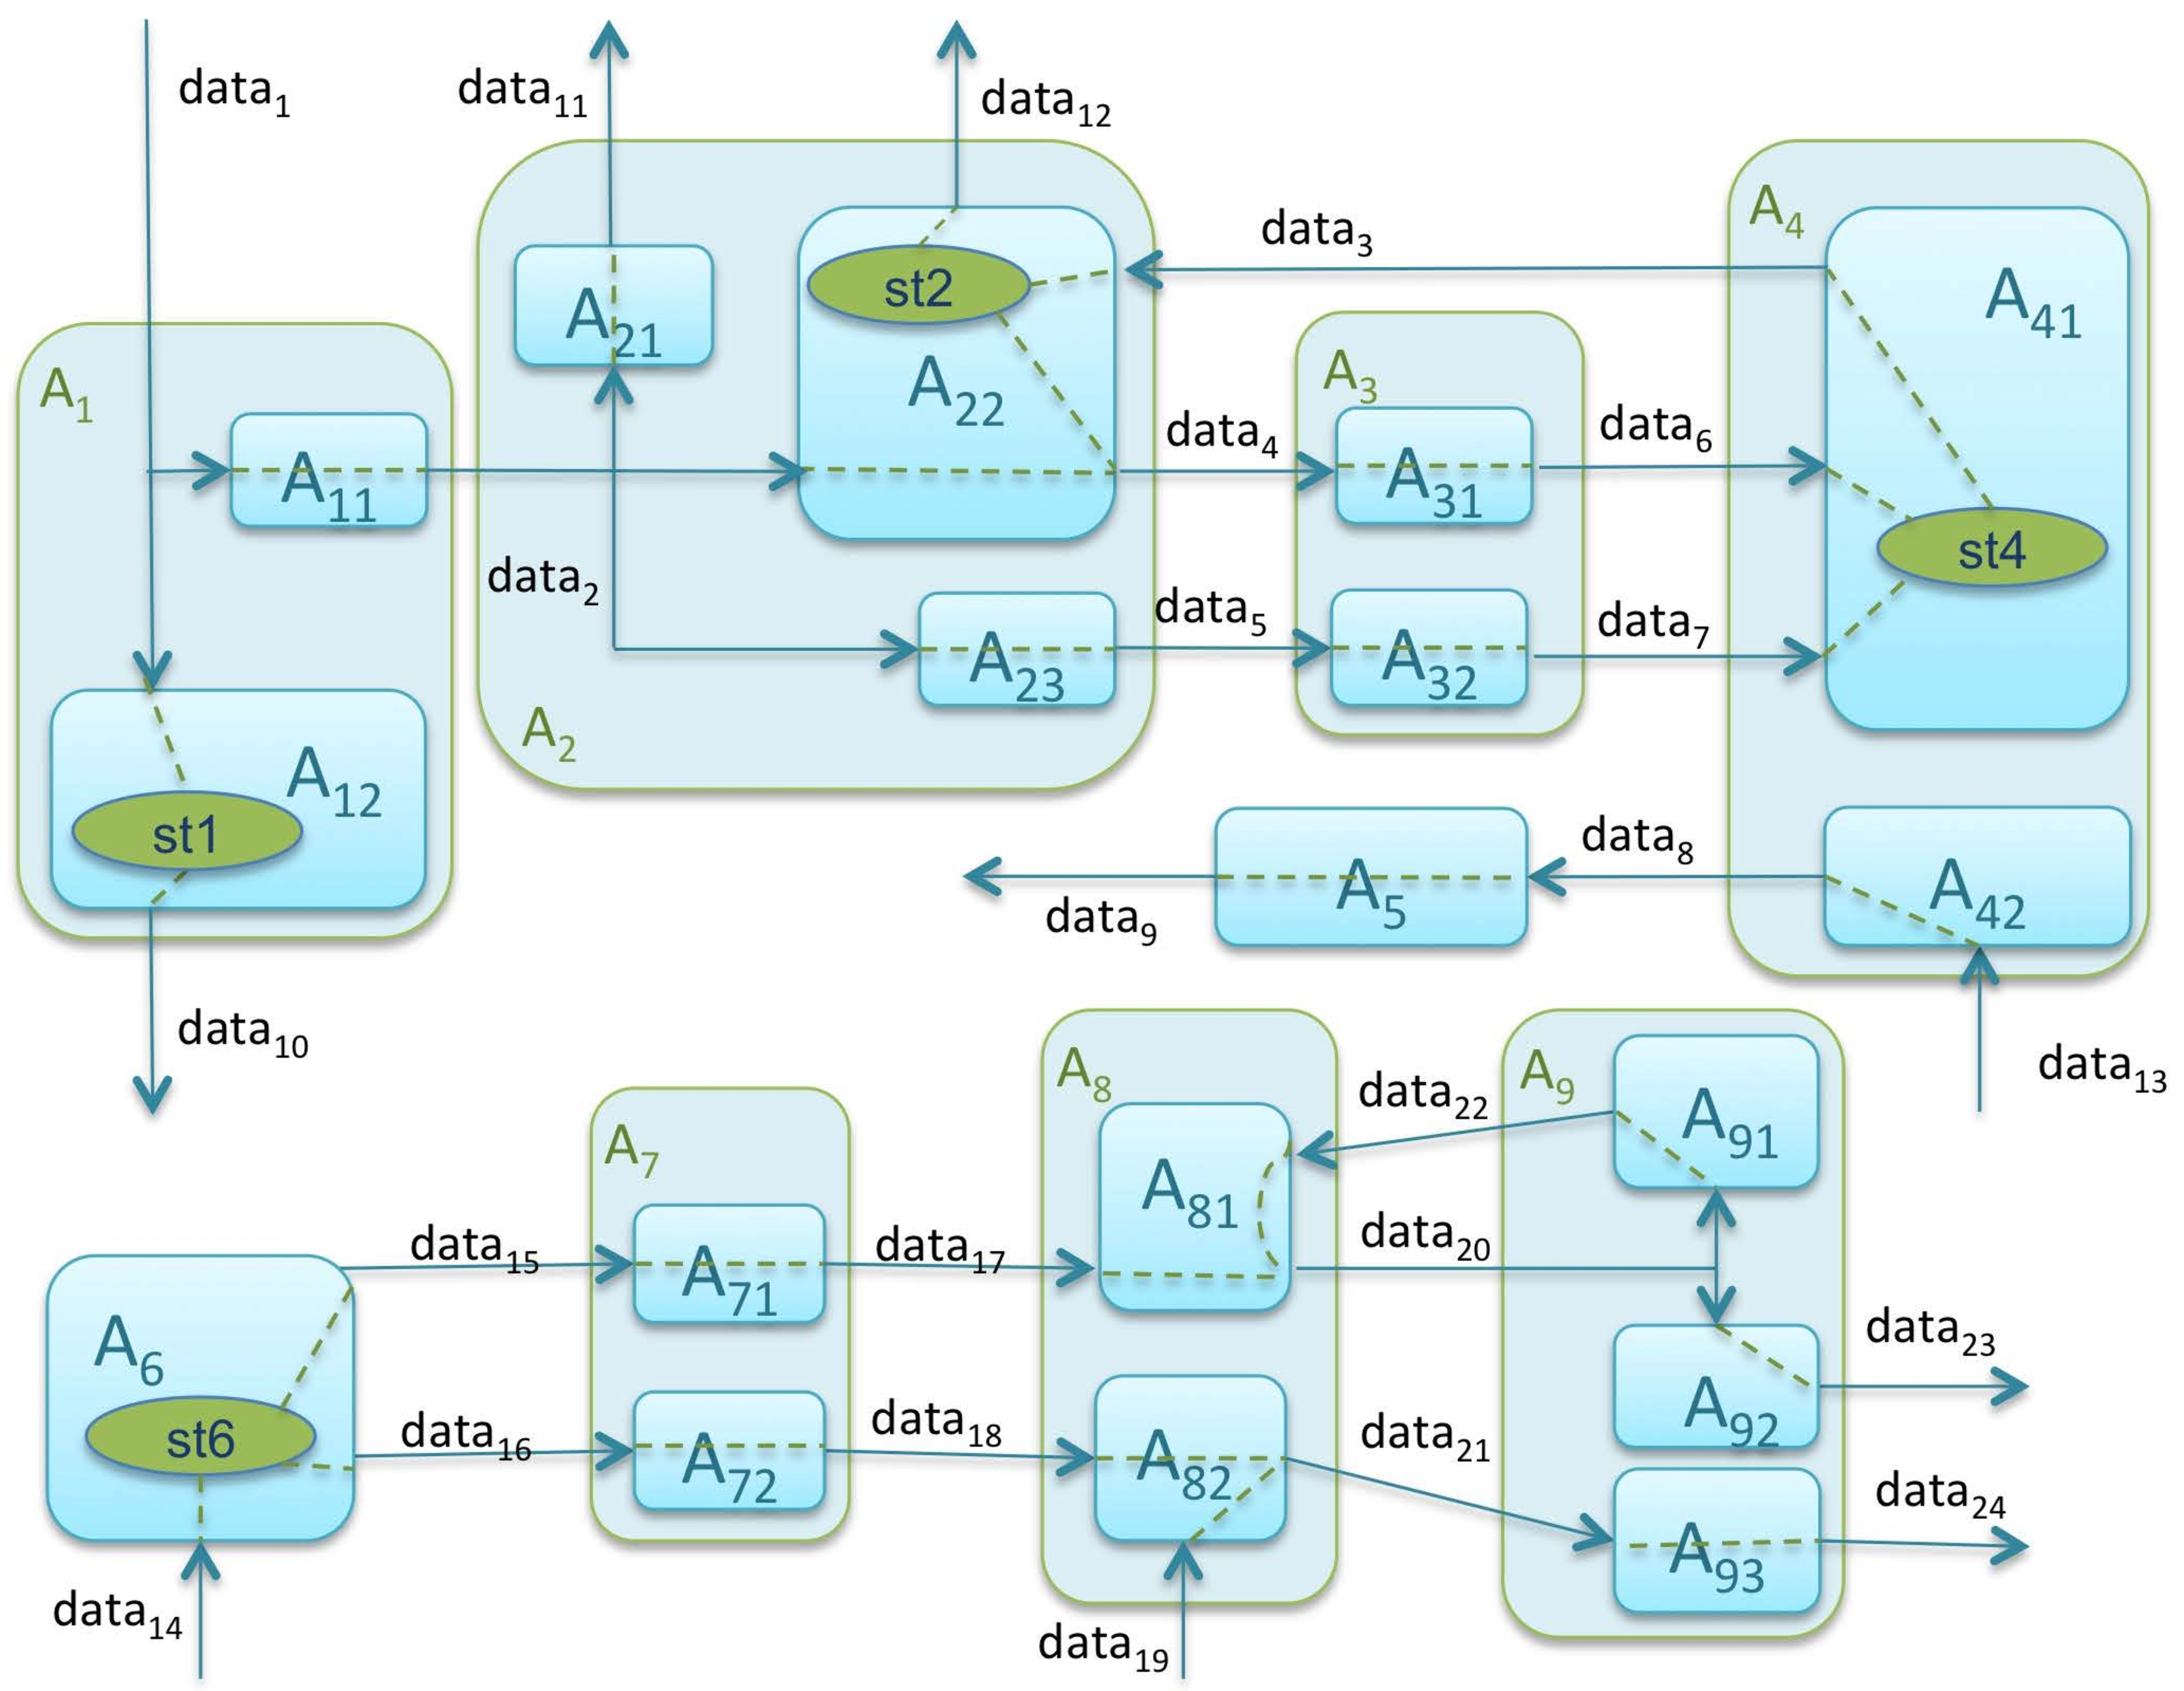
\includegraphics[scale=0.15]{fig/L1.pdf}
      \vspace{-2mm}
    \caption{% 
    Components' decomposition (level $L_{1}$)}
    \label{fig:example_comm2}
  \end{center}
\end{figure}

 \newpage
For each channel and elementary component 
(i.e. for any component on the abstraction level $L_{1}$) we specify the following measures:
\begin{itemize}
\item
measure for costs of the data transfer/ upload to the cloud \emph{UplSize(f)}:\\
 size of  messages (data packages) within a data flow $f$ and  frequency they are produced. 
This measure can be defined on the level of logical modelling, 
where we already know the general type of the data and 
can also analyse the corresponding  component (or environment) model to estimate the frequency the data are produced;
\item
measure 
for requirement of using high-performance computing and cloud virtual machines, \emph{Perf(X)}: 
complexity of the computation within a component $X$, which can be estimated on the  level of logical modelling as well.  
\end{itemize}
%
On this basis, we build a system architecture, optimised for remote computation.  
The \emph{UplSize} measure should be analysed only for the channels that aren't local for the components on abstraction levels $L_{2}$ and $L_{3}$.

\newpage
Using graphical representation, we denote the channels with \emph{UplSize} measure higher than a predefined value by thick red arrows (cf. also set \emph{UplSizeHighLoad} in
Isabelle theory \emph{DataDependenciesConcreteValues.thy}), and 
the components with  \emph{Perf} measure higher than a predefined value by   light green colour (cf. also set \emph{HighPerfSet} in
Isabelle theory \emph{DataDependenciesConcreteValues.thy}), 
where all other channel and components are marked  blue. 

Fig.~\ref{fig:remote} represents a system architecture, optimised for remote computation:
components from the abstraction level $L_{2}$ are composed together on the abstraction level $L_{3}$, if they are connected by at least one channel
 with \emph{UplSize} measure higher than a predefined value. 
The components $S_{4}'$ and $S_{7}'$ have  \emph{Perf} measure higher than a predefined value, i.e. using high-performance computing and cloud virtual machines is required.
\\
~
 
\begin{figure}[ht!]
  \begin{center}
   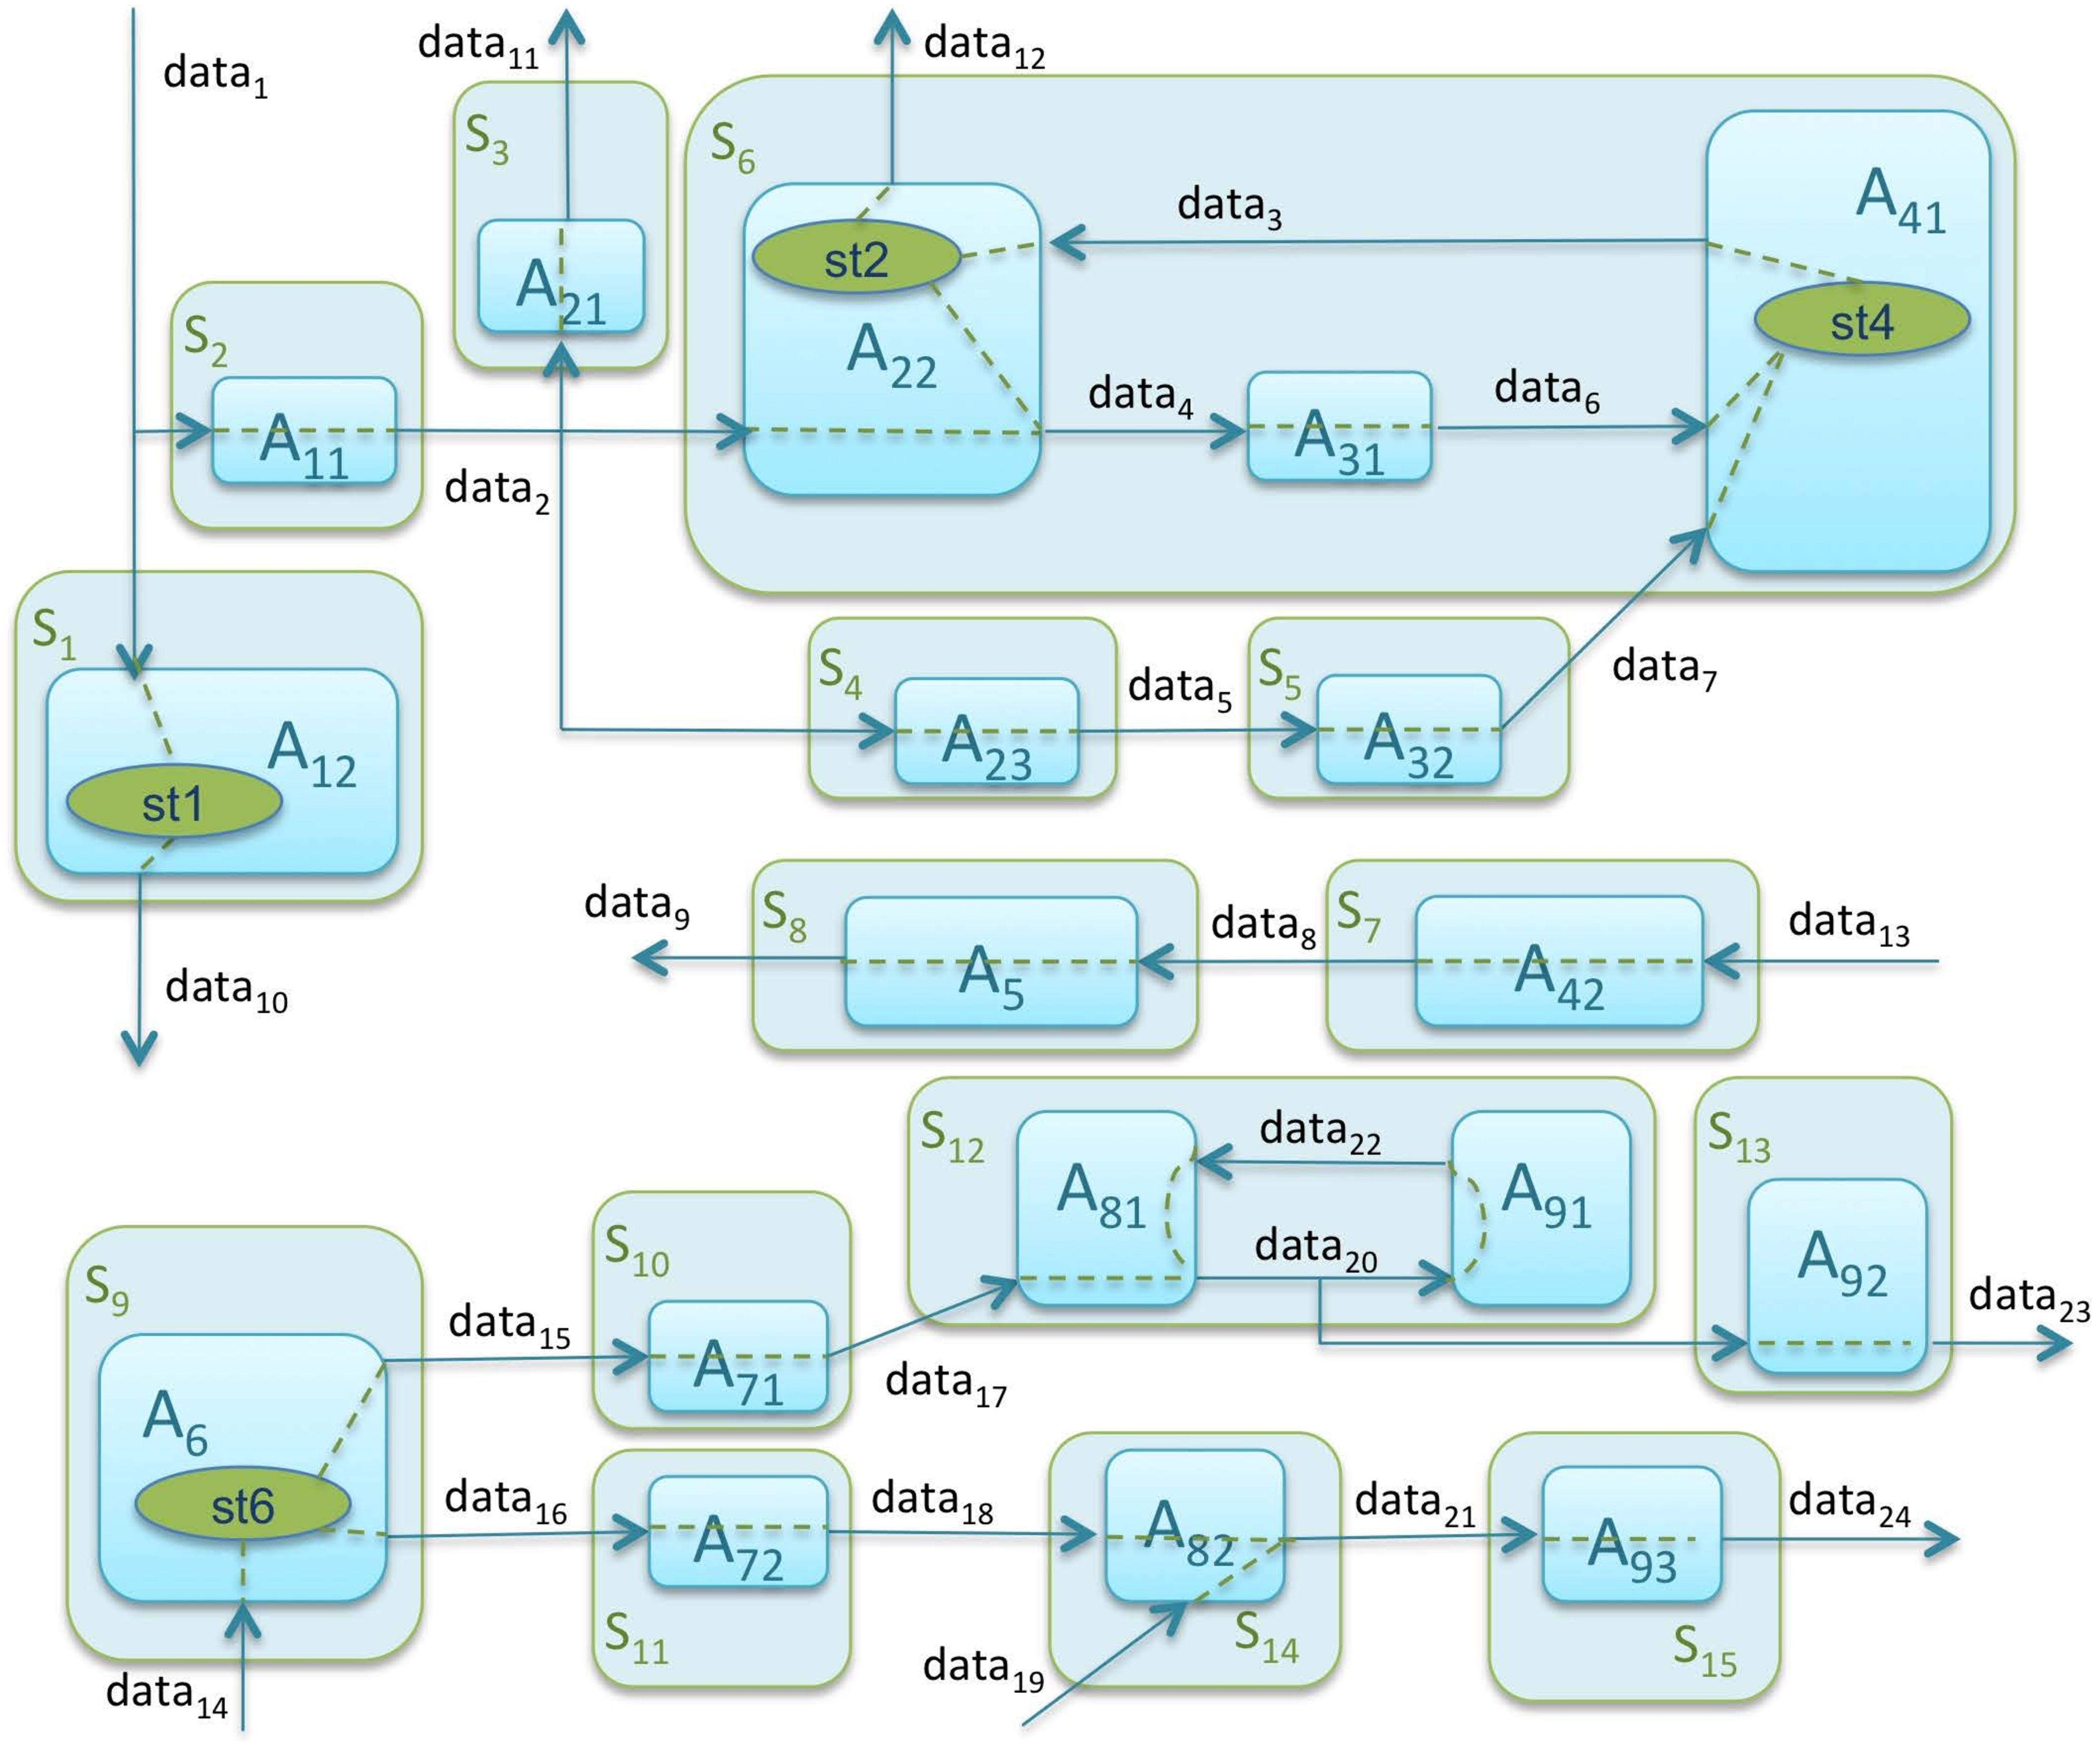
\includegraphics[scale=0.15]{fig/L2a.pdf}
    \caption{% 
    Architecture of $S$ (level $L_{2}$)}
    \label{fig:L2a}
  \end{center}
\end{figure}
 

 

\begin{figure}[ht!]
  \begin{center}
   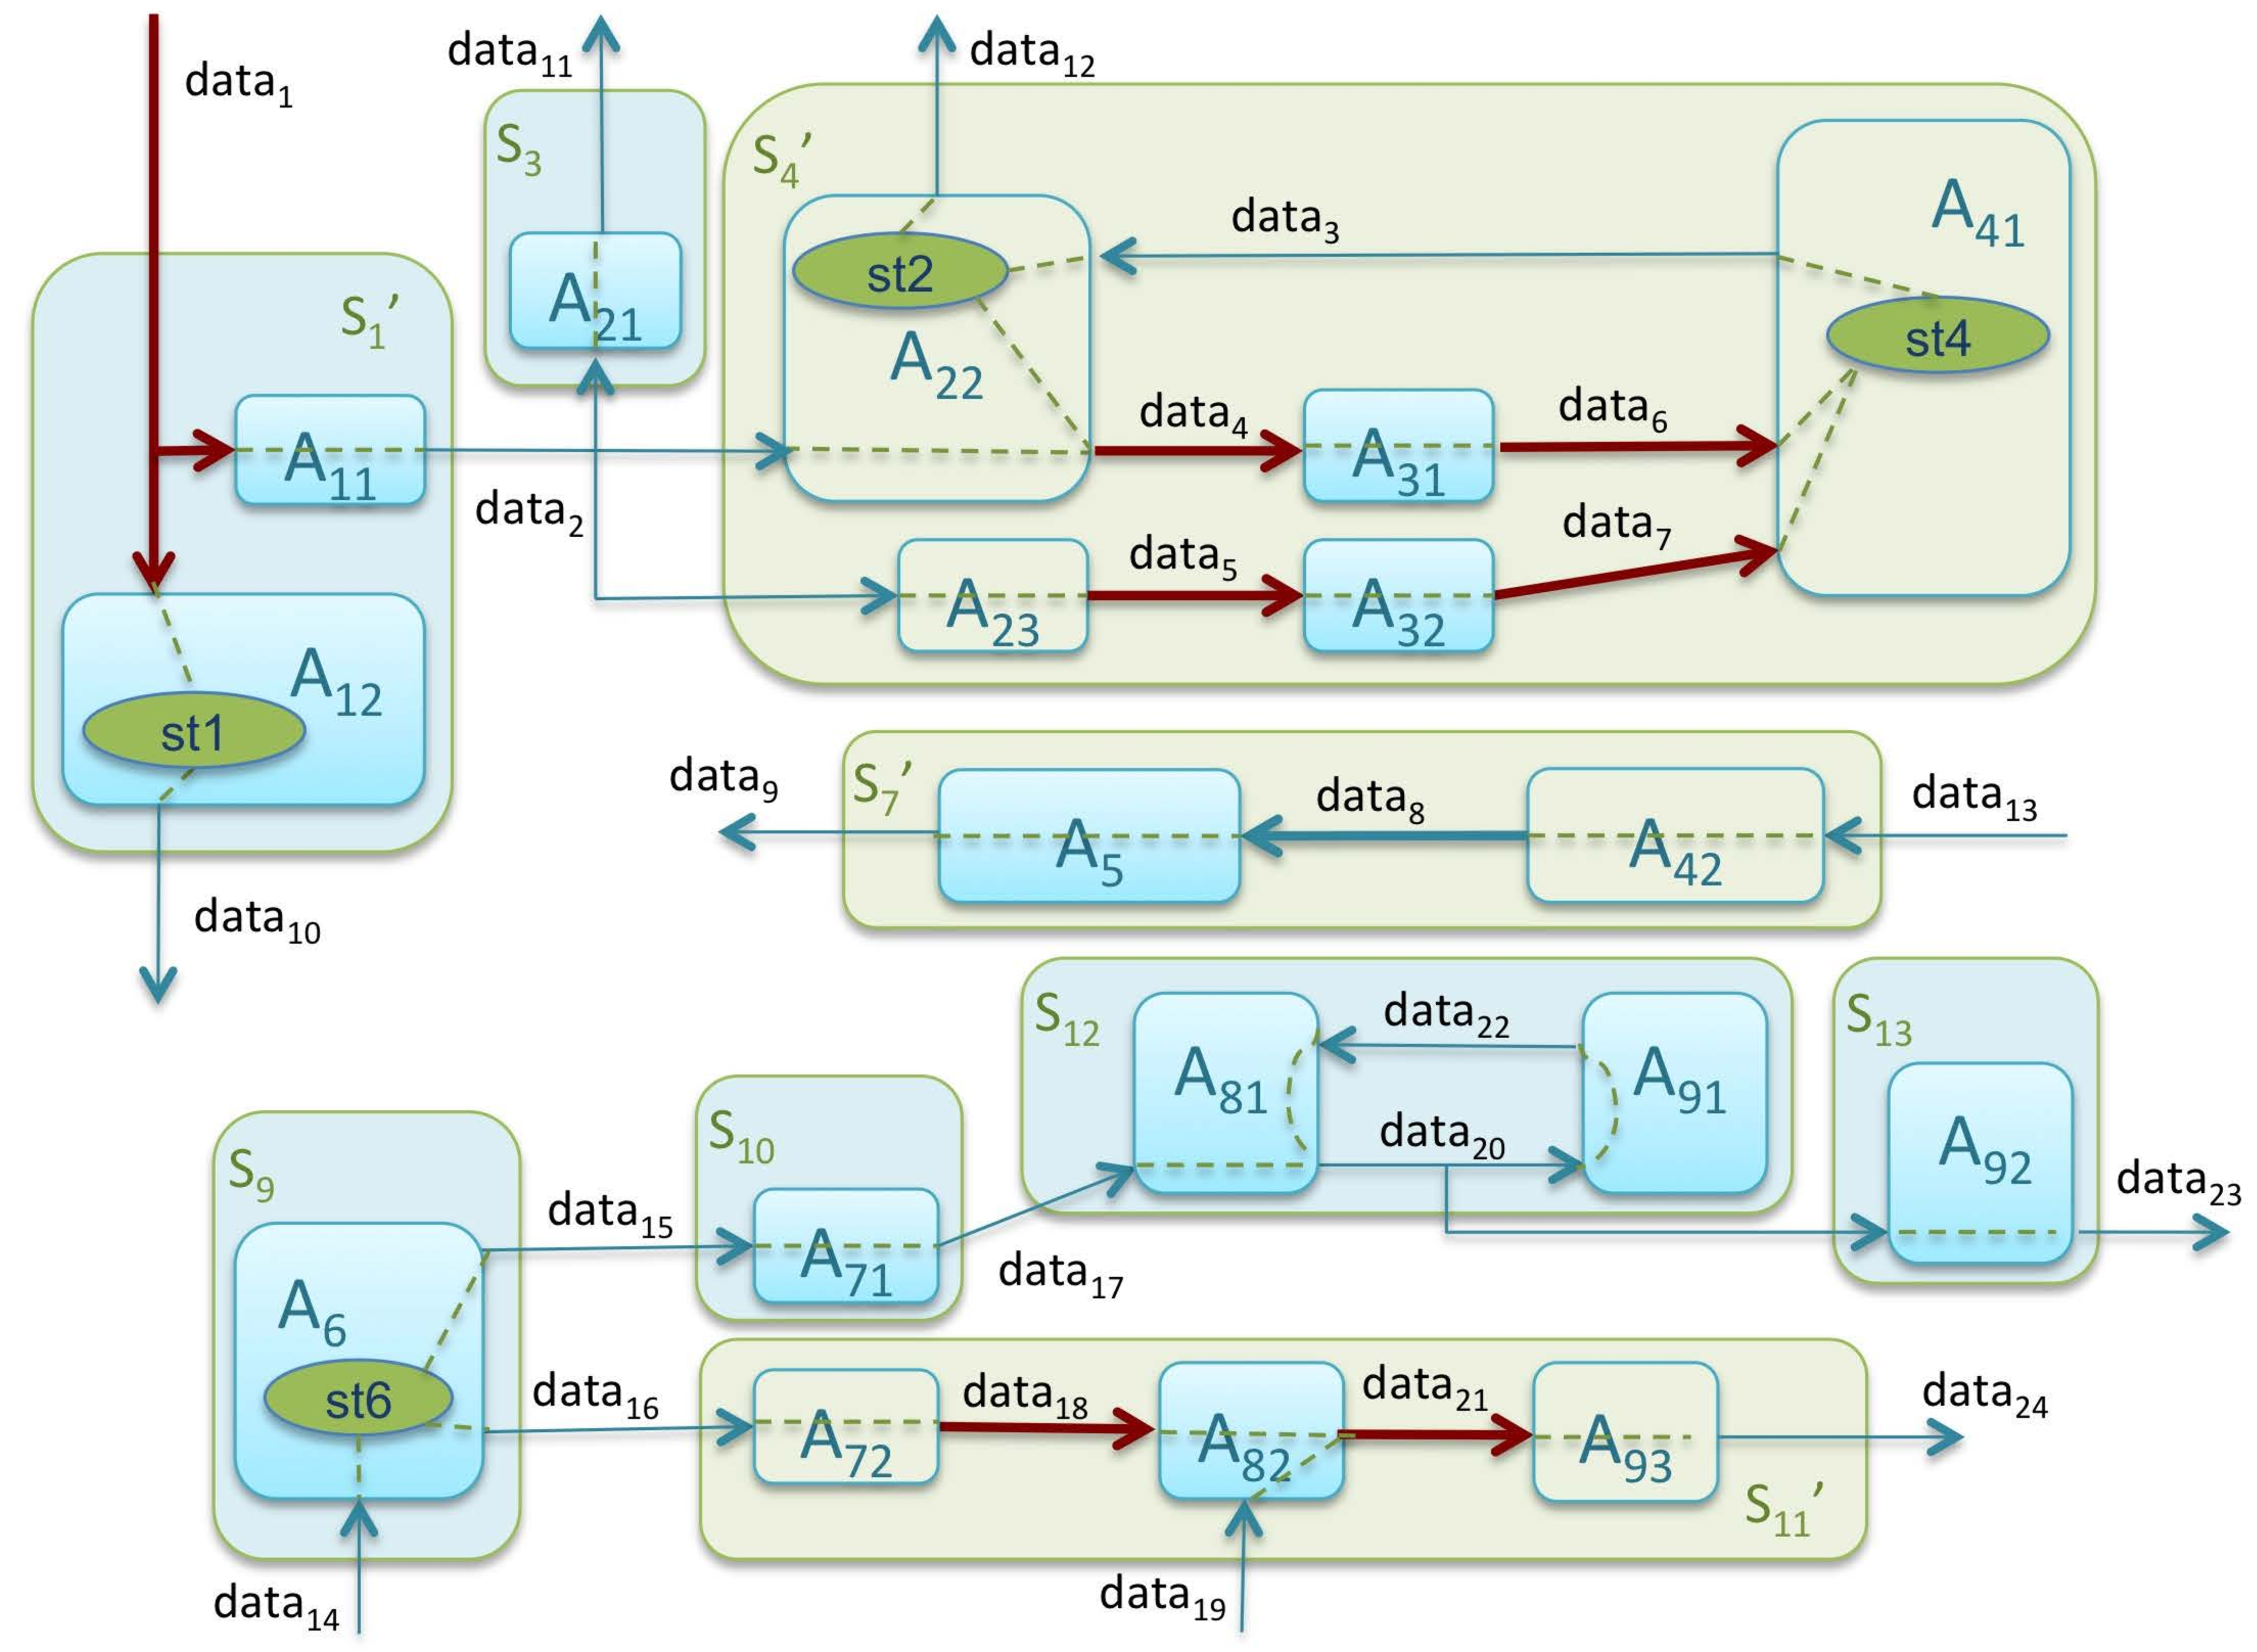
\includegraphics[scale=0.15]{fig/remote.pdf}
    \caption{%
    Optimised architecture of $S$  (Level $L_{3}$)}
    \label{fig:remote}
  \end{center}
\end{figure} 


